\section{Results and Discussion}
All three methods were applied to five meteorological variables across
all facilities. The methods identified different sets of outlier events,
with some events identified by more than one methods
(Figures~\ref{fig:pc},\ref{fig:ssa},\ref{fig:kmeans}).

Among three methods Pearson correlation was least effective with
frequent false negatives.
That is due to the fact that pairwise Pearson correlation method was 
applied at seasonal scale, thus was only able to find large outliers.
Pearson correlation coefficient is a pairwise comparison method, however, 
if the two variables deviates in the same direction, their correlation 
may not change significantly and thus may go undetected. Due to seasonal
nature of the analysis, it was not able to identify outliers that
persisted at hours to days only.
Univariate SSA method was very effective at identifying outlier high and
low values in the time series with high \textit{Precision} but low \textit{Recall}. 
$k$-means based outlier detection was also able to identify outliers
with high \textit{Precision} and low \textit{Recall}. 

\begin{table}[ht]
\caption{Comparison of SSA and K-means Outlier Set Size}
\label{tab:comp}
\centering
\begin{tabular}{|l|c|}
\cline{2-2}
\multicolumn{1}{l|}{} & Outlier Set Size\\
\hline
SSA & 922\\
K-means & 508\\
Intersection & 378\\
Symmetric Difference & 674\\
\hline
\end{tabular}
\end{table}

\begin{table}[ht]
\caption{Precision and Recall of SSA and K-means}
\label{tab:pr}
\centering
\begin{tabular}{|l|c|c|c|}
\hline
Method & Variable & Precision & Recall\\
\hline
SSA & temp\_mean & 16.00\% & 1.20\%\\
SSA & vapor\_pressure\_mean & 20.70\% & 1.40\%\\
SSA & atmos\_pressure & 0.00\% & 0.00\%\\
SSA & rh\_mean & 14.80\% & 0.50\%\\
SSA & wspd\_arith\_mean & 0.60\% & 1.50\%\\
Kmeans & 5 together & 12.90\% & 1.90\%\\
Combined & 5 together & 11.10\% & 4.10\%\\
\hline
\end{tabular}
\end{table}

SSA method identified largest number of outlier events (922)
(Table~\ref{tab:comp}) across the entire dataset, while $k$-means
identified 508 events. While 378 events were identified as outlier by
both the methods (intersection), 674 events were only identified by one
of the methods (Table~\ref{tab:comp}).
Figure~\ref{fig:combined} show all the outliers detected by SSA and
$k$-means methods at facility E33 for \textit{temp\_mean}. 
When combined together developed outlier detection methods had
\textit{Precision} of 11.10\% which show that many of the outliers
detected are not within ARM DQR database, which is a know limitation of
the current records that this current study is trying to address.
Detected outliers also had low \textit{Recall} which in addition to small
number of true positives can be due to fact that DQR database often
record a wide affected date range for an identified outlier instead of a
precise date thus leading to large false negatives, all of which leads
to low \textit{Recall} values.

Overall, when combined together within a framework, set of methods applied allows
to capture outlier events caused by a wide range of conditions. 

\begin{figure*}[ht]
    \centering
    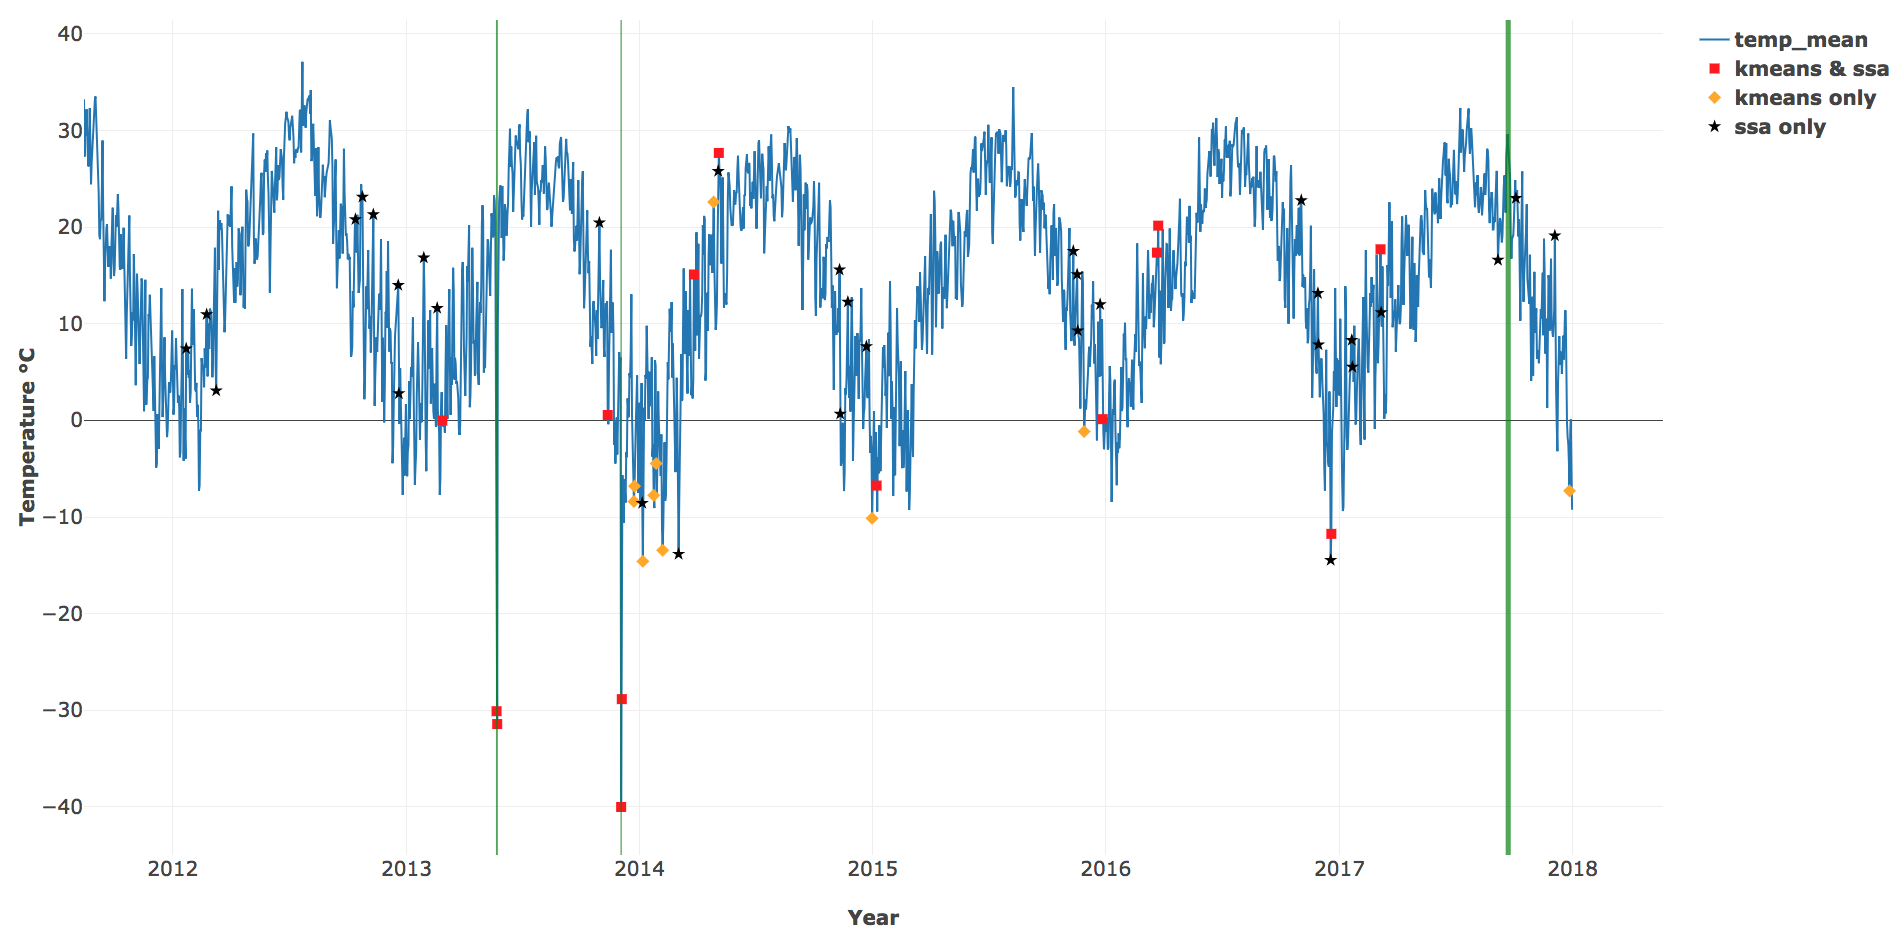
\includegraphics[width=\textwidth]{figures/combined.png}
    \caption{Outliers detected at facility E33 for \textit{temp\_mean}
		by SSA and $k$-means algorithms. Outliers detected by both
		algorithms are shown by red squares, while those identified by
		SSA and $k$-means only are indicated by black stars and orange
		diamonds respectively. DQR records are denoted by the vertical green shaded areas.}
    \label{fig:combined}
\end{figure*}
